\thispagestyle{empty}
\begin{titlepage}
    
\includegraphics[width=0.25\textwidth]{src/CoverPage/Deakin_Logo.jpeg}
        \begin{center}
        \vspace*{4cm}
        {\LARGE Investigation of Barren Plateaus in Quantum Neural Network Development}
        \vspace{3cm}
            \begin{large}   
    
        
            \bf Literature Review Draft
            \vspace{1cm}
        
            \bf \today \\
            T1-2022        
        
            \vspace{3cm}
            \textbf{Thanh Nguyen}\\
            STUDENT ID 218583133 \\
            COURSE - Bachelor of IT Honours (S470)
            \vfill

            \bf \normalsize Supervised by: Prof, Jacob Cybulski\\
       
        \end{large}  
   \end{center}
\end{titlepage}


\tableofcontents
\pagebreak

\todo{expect the audience to have some knowledge in QC, Linear algebra, ML}
\section{Overview}
This paper reviews the Quantum Neural Networks and Variational Quantum Algorithms, their structures, and the mathematics underneath. 
We aim to explore their gaps in studies, especially the factors that would lead to the problem of Barren Plateaus.
Then, we review and compare some methods to counter minimise the Barren Plateaus phenomenon by addressing those factors.

In general, Barren Plateaus can be noise-induced \cite{wangNoiseinducedBarrenPlateaus2021}, which means that the noise from quantum hardware affects the trainability; 
or circuit-induced \cite{mccleanBarrenPlateausQuantum2018}, as a result of the circuit design and initialisation parameters.
This research focuses on mitigating the effect of circuit induced Barren Plateaus by reviewing some of the available studies \cite{pesahAbsenceBarrenPlateaus2021, cerezoCostFunctionDependent2021, skolikLayerwiseLearningQuantum2021}.
From this point onward, we will address the term 'Noise-Induced Barren Plateaus' as 'Barren plateaus' for simplicity.

We strongly recommend readers to have foundation knowledge in Quantum Computing, Linear Algebra and Machine Learning. 
The 2020 Qiskit course \cite{2020QiskitGlobal} is a good start for beginners, this course provide very basic mathematics, theories and practices. 
The book \cite{sutorDancingQubitsHow2019} by Robert S. is also recommended while taking the 2020 Qiskit course, other than the basics of Quantum Computing, the author presented an overview of the current quantum hardware and simulator

\subsection{VQA and QNN}
\label{VQA}

Hybrid techniques involving quantum circuits and classical optimisers have been proposed to overcome the restrictions of Noisy Intermediate-Scale Quantum (NISQ) \cite{brooksQuantumSupremacyHunt2019} devices.
Those restrictions include inability of NISQ devices to achieve fault-tolerance, restrictions on the number of the available qubits per their quantum processors, and the limited depth of practically executable quantum circuits.
Moreover, quantum circuits and their gates are static by design, which means that input data into a quantum algorithm must be encoded as gates of the circuit implementing this algorithm. This implies that each instance of quantum algorithm use results in a new and distinct quantum circuit. This creates a barrier to using quantum circuits in support of efficient algorithm optimisation and training of quantum machine learning models.

Nevertheless, hybrid techniques, which combine classical and quantum techniques, allow development of \emph{variational circuits} (or circuit templates) with trainable parameters that can be iteratively refined by instantiating their values to create a static circuit using a traditional (classical) computer (i.e. when training VQAs) \cite{cerezo2021variational}, but which can then be efficiently executed on a quantum machine.
In this way, it is also possible to rely on range of classical optimisers, which treat variational circuits as black boxes capable of yielding outputs from inputs and the trainable parameters.

Consider a simple problem that we want to solve using VQA, given access to the training data.
The first step is to construct a \textit{cost function} $C$ used to search for an optimal set of circuit parameters, which is achieved by minimising the cost function during the training process.
We can simplify the development of variational circuits by composing the circuit templates called \textit{ansatze}.
\textit{Ansatz} is the parameterised circuit that depends on a set of parameters $\theta$. We aim to train the ansatze by optimising the parameters $\theta$s so that the cost function $C$ reaches its minimum, thus satisfying:
\begin{equation}
    \theta^* = \underset{\theta}{\arg \min} \;C(\theta)
    \label{optimize theta with ansatz}
\end{equation}

In short, the cost function $C(\theta)$ is calculated using the quantum computer, while the classical optimiser trains the parameters $\theta$. Figure \ref{VQA diagram} explains the VQA architecture and elaborates its training process in more detail.

\begin{figure}
    \centering
    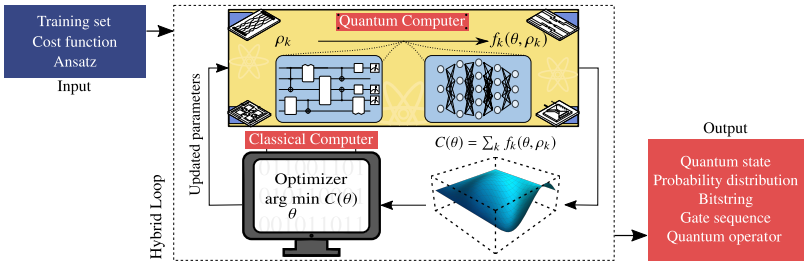
\includegraphics[width=\textwidth]{LiteratureReview/Appendices/vqadiagram.png}
    \caption{
        An illustrative diagram of VQA.
        The algorithm is a hybrid loop that receives:
        A cost function $C(\theta)$ for $\theta$ is a set of parameters that encodes the solution;
        An ansatz that receives trainable parameter $\theta$ to solve the task;
        A set of training data $\{\rho_k\}$.
        We use the quantum computer to calculate the cost for each iteration, then use an optimisation algorithm in a classical computer to find the global minima in the cost landscape $C(\theta)$ and thus satisfy the problem in Eq. (\ref{optimize theta with ansatz}).
        VQA's result is an approximation of the problem solution, which can take forms as in the red box.
        Figure from Cerezo et al. \cite{cerezo2021variational}.
    }
    \label{VQA diagram}
\end{figure}

\subsubsection{The Cost Function}
Encoding the problem into a cost function is the first step in solving a problem using VQA \cite{cerezo2021variational}.
The cost function is equivalent to that used in classical machine learning.
It maps the values of the trainable parameters $\theta$ into real values, which represent the measure of distance from an optimum solution.
For a function $f$ that receives input states $\{\rho_k\}$, observables $\{O_k\}$, and a parameterized circuit $U(\theta)$, the cost is expressed as:
\begin{equation}
    C(\theta) = f(\{\rho_k\}, \{O_k\}, U(\theta)) \;,
\end{equation}
or this form with a set of functions $\{ f_k \}$ and the square of a distance matrix given as its trace $Tr$:
\begin{equation}
    C(\theta) = \sum_k f_k \left(\Tr[ O_k U(\theta) \rho_k U^\dagger(\theta) ]\right) \;,
    \label{Cost function}
\end{equation}

For the function to be used as a cost function it must meet a number of criteria:
(1) The cost function must be 'faithful' and 'operationally meaningful', such that the minimum of $C(\theta)$ should correspond to the solution of the problem, and the lower cost function indicate a better solution in general;
(2) Cost function must be 'efficiently estimable' by the measurement conducted on a quantum computer and the subsequent classical post-processing;
(3) The cost must be 'trainable', such that the parameters $\theta$ could be efficiently optimised.

\subsubsection{Ansatze}
\begin{figure}
    \centerline{
    \Qcircuit @C=1em @R=0em {
    & \multigate{2}{U_1(\theta_1)}    & \multigate{2}{U_2(\theta_2)}    & \qw &        & & \multigate{2}{U_L(\theta_L)}   & \qw\\
    & \ghost{U_1(\theta_1)}           & \ghost{U_2(\theta_2)}           & \qw & \cdots & & \ghost{U_L(\theta_L)}          & \qw\\
    & \ghost{U_1(\theta_1)}           & \ghost{U_2(\theta_2)}           & \qw &        & & \ghost{U_L(\theta_L)}          & \qw
    \gategroup{1}{2}{3}{7}{.6em}{--}
    }
    }
    \centerline{$U(\theta)$}
    \centerline{}
    \centerline{}
    \centerline{
    \Qcircuit @C=1em @R=0em{
    & \multigate{1}{}   & \ctrl{2}  & \gate{}           & \qw \\
    & \ghost{}          & \qw       & \multigate{1}{}   & \qw \\
    & \gate{}           & \targ     & \ghost{}          & \qw
    \gategroup{1}{2}{3}{4}{.6em}{--}
    }
    }
    \centerline{$U_l(\theta_l)$}
    \caption{
        A diagram of a sample ansatz (above), the ansatz is a sequence of unitaries $U_l(\theta_l)$ (below).
        The unitary $U(\theta)$ receives parameters $\theta$ is expressed by $L$ layers of unitaries $U_l(\theta_l)$ for $l$ is the layer indices.
        Each $U_l(\theta_l)$ is a circuit composed of a mix of parameterised and unparametrised gates.
    }\label{Ansatz diagram}
\end{figure}

In physics and mathematics, \emph{ansatz} (plural \emph{ansatze}) is an educated guess or a starting point from which you start looking for a solution to the problem at hand. In quantum computing, \emph{ansatz} is a parameterised circuit, formed as a sequence of unitary (or "atomic") circuits, which is used as a framework for the circuit optimisation.
In general, the location of parameters $\theta$ is determined by the ansatz form and can be trained to minimise the cost.
The ansatz structure can be defined based on the problem (called 'problem-inspired ansatze') or a generic structure (called 'problem agnostic ansatze') that can be used without any relevant information available \cite{cerezo2021variational}.

The cost function in Eq. (\ref{Cost function}) encodes the parameters $\theta$ in a unitary $U(\theta)$ and applies to the input states of the circuit.
The figure \ref{Ansatz diagram} shows that $U(\theta)$ can be expressed as a product of $L$ consecutive unitaries:
\begin{equation}
    U(\theta) = U_L(\theta_L) \cdots U_2(\theta_2) U_1(\theta_1)\;,
\end{equation}
with each layer:
\begin{equation}
    U_l(\theta_l) = \prod_m e^{-i\theta_m H_m} W_m
\end{equation}
for unparamaterized unitary $W_m$, hermitian operator $H_m$, and $\theta_l$ is the $l$-th element of $\theta$.

\subsubsection{Gradients}
After defining the cost function and a suitable ansatz, we train the parameter $\theta = \{\theta_{l}\}$ to solve the problem in Eq. (\ref{optimize theta with ansatz}) \cite{cerezo2021variational}.
The cost function gradient helps the optimiser to find the global minima.
Consider the cost function in Eq. (\ref{Cost function}), for a unitary that parameterises rotation $e^{i \theta_l \sigma_{l}}$, where $\theta_l$ be the $l$-th element of $\theta$, $\sigma_l$ is a Pauli rotation operator.
We can evaluate the gradient with the parameter-shift rule:
\begin{equation}
    \frac{\partial C}{\partial\theta_l}
    = \sum_k \frac{1}{2 \sin{\alpha}}
    \left(
    \Tr[O_k U^\dagger(\theta_+) \rho_k U(\theta_+)]
    - \Tr[O_k U^\dagger(\theta_-) \rho_k U(\theta_-)]
    \right) \;,
    \label{Parameter-shift rules}
\end{equation}
with $\theta_{\pm} = \theta \pm \alpha e_l$, $\alpha \in \mathbb{R}$ and $e_l$ is a vector such that its $l$-th position have the value of 1, or else 0.

Essentially, we can shift the $l$-th parameter by some amount $\alpha$, and Eq. (\ref{Parameter-shift rules}) will calculate the gradient.


\subsubsection{Optimisers}
The accuracy of VQA greatly depends on the optimisation method.
Typically, we can achieve the solution by making successive moves along the gradient direction.
This optimisation approach is within the scope of stochastic gradient descent (SGD).
One example of SGD is the ADAM optimiser \cite{kingmaAdamMethodStochastic2014}, which can vary the size of the steps taken during optimisation to produce more efficient and precise results compared to the basic SGD.


\subsubsection{About QNN}
VQA is also the most widely used method for developing Quantum Neural Network (QNN) circuits.
As a result, QNN inevitably inherited some of VQA's features and flaws.
Many quantum machine learning models suffer from the issue of \textit{barren plateaus} \cite{zhaoReviewQuantumNeural2021} that prevent the growth of circuit depth and lead the training of parameters to a dead end.
When training a QNN framework with a large number of qubits, this phenomenon is likely to occur; the objective function becomes flat, whereby its gradient is nearly zero across a large plateau, making it nearly impossible to identify the global minimum (also defined by the zero gradient), \cite{mccleanBarrenPlateausQuantum2018, zhaoAnalyzingBarrenPlateau2021} causing inefficiency in circuit training.
We will discuss this matter in later sections.

% Some architectures of QNN have been proposed to counter this problems, for example: 
% Quantum Tensor Neural Network (QTNN) \cite{hugginsQuantumMachineLearning2019} which achieved a balance of computational efficiency and expressive power. 
% The tensor network can reduce the required number of qubits to process high-dimensional data with powerful optimisation algorithms.
% An alternative solution is to rely on Quantum Recurrent Neural Network (QRNN) which is constructed as a parameterised circuit \cite{takakiLearningTemporalData2021}, with some qubits being initialised and measured at each step while others memorise the past data.

Many types of QNN models also suffer from the emergence of barren plateaus during their training (although for different reasons), for example in:
Quantum Boltzmann Machines \cite{shinguBoltzmannMachineLearning2021, zoufalVariationalQuantumBoltzmann2021},
Quantum Perceptrons \cite{kristensenArtificialSpikingQuantum2021} and
Quantum Generative Adversarial Networks \cite{dallaire-demersQuantumGenerativeAdversarial2018, lloydQuantumGenerativeAdversarial2018}.
It is worth noting that Quantum Convolutional Neural Networks (QCNNs) do not exhibit barren plateaus \cite{pesahAbsenceBarrenPlateaus2021}.
Thus, training convergence is more successful for QCNNs under random initialisation.

Studies have shown that Neural Network training and execution performance involving quantum machines can be significantly higher than that achievable using today's classical hardware \cite{abbasPowerQuantumNeural2021, colesSeekingQuantumAdvantage2021}. Consequently quantum neural nets may find some promising applications, for example, in breast cancer prediction \cite{liModelAlgorithmQuantuminspired2014} or image processing \cite{matsuiQubitNeuralNetwork2009}.

\subsection{Barren Plateaus, Gradients, Trainability Issue} \label{Barren Plateaus section}

When training a quantum circuit, three important elements are needed to construct the initial variational circuit and a cost function: some reference states (the inputs), a parameterised unitary operation (the circuit, or ansatz), and an observable $O$ (the outputs). Then we also need to select a suitable classical optimiser.

The next step is to evolve this variational circuit from the initially random state of circuit parameters to the circuit instantiated with the optimal parameter values.

The process is iterative. At each cycle of the optimisation, the optimiser suggests the values for the variational circuit parameters, optionally increases the circuit depth, instantiates the circuit with the parameters values, and runs thus created executable circuit on a quantum machine.
The obtained outputs can subsequently be compared with the observables and the current value of the cost function calculated, so that the optimisation routine could then suggests the new set of parameters for the evolving circuit \cite{cerezo2021variational}.
By changing the circuit parameters, we are exploring an optimisation landscape to find a global minimum for the cost function, and thus the optimum circuit parameters.
The properties of this landscape heavily depend on the structure of the parameterised circuit (derived from input-output pairs and the selected ansatz) and the selected cost function.

Typically, two starting ingredients for problem-solving using heuristic ansatzes are a randomly parameterized circuit $U$ and a set of random initialization parameters $\vec{\theta}$, non-parameterized unit $W_l$ for each layer $l$ \cite{mccleanBarrenPlateausQuantum2018}:
\begin{equation}\label{Parameterized Circuit}
    U(\vec{\theta})
    = U(\theta_1, \cdots, \theta_L)
    = \prod_{l=1}^L U_l(\theta_l)W_l
\end{equation}
With $L$ is the depth of the circuit. Consider a cost function $C(\theta)$ with an observable $O$ and the ansatz $U$:
\begin{equation}
    C(\vec{\theta})
    = \bra{0} U(\vec{\theta})^\dagger OU(\vec{\theta}) \ket{0}
\end{equation}

The gradients are the derivatives of the cost function respectively to the parameters and have a severe impact on the performance of the training model:
\begin{equation}
    \partial_l C = \frac{\partial C(\vec{\theta})}{\partial\theta_l}
\end{equation}
McClean et al. \cite{mccleanBarrenPlateausQuantum2018} also pointed out that whenever the random parameterised circuits reach the depth $O(n^{1/L})$ on a $L$-dimensional array, the gradient of the cost function will vanish.
The variance of the gradient shrinks exponentially with the number of qubits $n$:
\begin{align}
    \langle \partial_k C\rangle & = 0  \label{Vanish Gradient}                  \\
    \mathrm{Var}[\partial_k C]  & \approx 2^{-n}  \label{Variance expo smaller}
\end{align}
Barren plateaus is a serious issue for circuit optimisation because the flatter the landscape is, the more challenging it is to search for the location of the global cost minimum.
Compared to the gradient in a deep classical network which vanishes exponentially in the number of layers, for the QNN case, the gradient grows exponentially small with the number of qubits \cite{mccleanBarrenPlateausQuantum2018}.

Additionally, the choice of the initiate parameter $\theta$ is also an important factor. When an ansatz is randomly initialised, the algorithm may start far from the solution, at a local minimum, or even on the surface of a barren plateau.

To summarise, the following factors can lead to barren plateaus in QNN and VQA:
\begin{itemize}
    \item \textbf{\emph{The ansatz depth and the number of qubits}}
    \item \textbf{\emph{Random initialization parameters}}
\end{itemize}



\subsection{Addressing Parameterized circuit depth}
\subsubsection{Shallow Circuits, Local Cost Function}
\begin{figure} 
    \centerline{
        \Qcircuit @C=1em @R=0em {
        & \multigate{4}{U(\theta)}    & \meter\\
        & \ghost{U(\theta)}           & \meter\\
        & \ghost{U(\theta)}           & \meter\\
        & \ghost{U(\theta)}           & \meter\\
        & \ghost{U(\theta)}           & \meter\\
        }
    }
    \centerline{a) Global Cost Function}
    \centerline{
        \Qcircuit @C=1em @R=0em {
        & \multigate{4}{U(\theta)}    & \meter\\
        & \ghost{U(\theta)}           & \qw\\
        & \ghost{U(\theta)}           & \qw\\
        & \ghost{U(\theta)}           & \qw\\
        & \ghost{U(\theta)}           & \qw\\
        }
    }
    \centerline{b) Local Cost Function}
    \caption{
        Global Cost Function and Local Cost Function.
        a) Global Cost Function compares the states in exponentially large Hilbert space.
        b) Local Cost Function compares the states at single qubit level.
    }\label{cost functions}
\end{figure}

Cerezo et al. has demonstrated \cite{cerezoCostFunctionDependent2021} properties of a 'local cost function' in a parameterised circuit. 
Let us recall the cost function $C$ with an operator $O$, the ansatz $U(\theta)$ and some input states $\rho$:
\begin{equation}
    C = \Tr\left[
    OU(\theta) \rho U^\dagger(\theta)
    \right],
\end{equation}
the authors called this cost function as 'Global Cost Function' $C_G$, which can inhabit Barren Plateaus. Compared to the proposed 'Local Cost Function':
\begin{equation}
    C_L = \Tr\left[
    O_L U(\theta) \rho U^\dagger(\theta)
    \right],
\end{equation}
with
\begin{equation}
    O_L = I- \frac{1}{n} \sum^n_{j=1}\rho_j \bigotimes I_{\overline{j}},
\end{equation}
where $I_{\overline{j}}$ is the identity on all qubits except the qubit in $j$-th position.



if a \almarginpar{Explain what is "local" vs "global" cost function}\underline{local cost} function is used, then there is a lower bound for the variants of the gradients that depends on the number of qubits and some configurations of the circuit. 
For a $L$-layered ansatz, let the variance $\mathrm{Var}[\partial_v C]$ of the partial derivative of the cost function $C$, the lower bound $G_n$ for the variance is:
\begin{equation}
    G_n(L,l) \leq \mathrm{Var}[\partial_k C]
\end{equation}
\begin{equation}
    G_n(L,l) = \frac{{2}^{m(l+1)-1}}{{({2}^{2m}-1)}^{2}{({2}^{m}+1)}^{L+l}}
    \times \mathop{\sum}\limits_{i\in {i}_{{\mathcal{L}}}}\mathop{\sum}\limits _{{(k,k^{\prime} )\in {k}_{{{\mathcal{L}}}_{\text{B}}}}\atop {k^{\prime} \geqslant k}}{c}_{i}^{2}\epsilon ({\rho }_{k,k^{\prime} })\epsilon ({\widehat{O}}_{i})\ ,
\end{equation}
Where the forward light-cone $\mathcal{L}$ is a set of gates with at least one input connected to the output of a block $W$; 
The backward light-cone $\mathcal{L}_\text{B}$ is a set of gates with at least one output connected to the input of block $W$;
$S_k$ is the $m$-qubit subsystem;
$i_{\mathcal{L}}$ is a set of indices such that the operators $\hat{O_i}$ act on qubits in $\mathcal{L}$;
$k_{\mathcal{L}_B}$ is a set of indices such that the subsystem $S_k$;

\almarginpar{What is $G_n$}If the total depth $L$ is in the range $O(\log(n))$ of the number of qubits (a shallow configuration), then the lower bound cannot vanish faster than $\Omega(1/\mathrm{poly}(n))$. 
Thus, no Barren Plateau occurs in this case.\almarginpar{You throw lots of formulas in but do not explain much}



\subsubsection{Layerwise learning for quantum neural networks}

There is another method that manipulates the circuit depth throughout the training period studied by Skolik et al. \cite{skolikLayerwiseLearningQuantum2021}. 
In more detail, the algorithm consists of two phases:

\almarginpar{Good find "qcircuit"!}\textbf{The first phase} constructs the ansatz by adding layers one by one, with the parameters are all initially zero. For a small number $s$ of starting layers, the set of parameters $\vec{\theta_1}$, and $W$ operators connecting qubits, then the initial layers $l_1(\vec{\theta_1})$ is presented:

\begin{equation}
    l_1(\vec{\theta_1})
    = \prod_{j=1}^s U_{1_j}(\vec{\theta_{1_j}}) W \;,
\end{equation}

Where each consecutive layer $l_i(\vec{\theta_i})$ of form
\begin{equation}
    l_i(\vec{\theta_i})
    =U_i(\vec{\theta_i}) W \;,
\end{equation}
is added after a certain number of epochs and the previous layers' parameters become fixed. 
One epoch is the set of iterations for the algorithm to see each training sample; an update of all trainable parameters is called one iteration.

This process can stop when a certain circuit depth is reached or until the objective function's value does not improve with additional layers.
Figure \ref{ll circuit} provides an illustrative example of the final circuit.
Eventually, we obtain the final circuit of $L$ layers:

\begin{equation}
    U(\vec{\theta})
    = \prod_{i=0}^L l_i (\vec{\theta_i}) \;.
\end{equation}
\begin{figure} 
    \centerline{
        \Qcircuit @C=1em @R=0em {
        & \multigate{4}{l_1(\vec{\theta_1})}    & \multigate{4}{l_2(\vec{\theta_2})}    & \qw &        & & \multigate{4}{l_i(\vec{\theta_i})}   & \qw\\
        & \ghost{l_1(\vec{\theta_1})}           & \ghost{l_2(\vec{\theta_2})}           & \qw &        & & \ghost{l_i(\vec{\theta_i})}          & \qw\\
        & \ghost{l_1(\vec{\theta_1})}           & \ghost{l_2(\vec{\theta_2})}           & \qw & \cdots & & \ghost{l_i(\vec{\theta_i})}          & \qw\\
        & \ghost{l_1(\vec{\theta_1})}           & \ghost{l_2(\vec{\theta_2})}           & \qw &        & & \ghost{l_i(\vec{\theta_i})}          & \qw\\
        & \ghost{l_1(\vec{\theta_1})}           & \ghost{l_2(\vec{\theta_2})}           & \qw &        & & \ghost{l_i(\vec{\theta_i})}          & \qw\\
        }
    }
    \caption{
        Constructing the ansatz from shallow layers.
    }\label{ll circuit}
\end{figure}


\textbf{The second phase} takes the pre-trained circuit from phase one and trains \almarginpar{What are these?}\underline{larger adjacent partitions} of layers at a time. 

\subsection{Addressing Random initialization parameters}

\subsubsection{Layerwise learning for quantum neural networks \texorpdfstring{\cite{skolikLayerwiseLearningQuantum2021}}{}}
The algorithm in \cite{skolikLayerwiseLearningQuantum2021} starts with training a shallow circuit to its best, then extends the circuit and uses the best parameter achieved in the previous step for the newly extended circuit. 
Note that only the new parameters are allowed to vary while the previous parameters are frozen.
Thus, the randomness is contained to only shallow sub-circuits in phase one during the whole routine and minimizes the probability of meeting a plateau during the process.


\subsubsection{An initialization strategy for addressing Barren Plateaus in parameterized quantum circuit \texorpdfstring{\cite{grantInitializationStrategyAddressing2019}}{}  }

Grant et al. have addressed the Random initialization parameter so that the early training steps do not start on a plateau region. 
The idea is to divide the big parameterized circuit into blocks and initialize each block so that the result is a fixed unitary matrix, i.e., an identity operation. 
The method is as follows: partition the circuit into $M$ blocks of depth $L$; for each block, initiate some parameters with random values, and fix the remaining parameters in a way that results in a fixed unitary matrix, i.e., invert the first part so that each block implements an identity operation.

The depth $L$ is chosen to be shallow enough so that each block cannot reach 2-designs. For any $m = 1, \cdots, M$, the parameters $\theta$, the block is presented as:
\begin{equation}
    U_m(\theta_m)
    = \prod_{l=L}^1 U_l(\theta_{l,1}^m) \prod_{l=1}^L U_l(\theta_{l,2}^m).
\end{equation}
The starting parameter $\theta_{l,1}$ can be chosen randomly, while the values for $\theta_{l,2}$ are chosen such that $U_l(\theta_{l,2}) = U_l(\theta_{l,1})^\dagger$:
\begin{equation}
    U_m(\theta_m)
    = \prod_{l=L}^1 U_l(\theta_{l,1}^m)
    \prod_{l=1}^L U_l(\theta_{l,1}^m)^\dagger
    = I_m,
\end{equation}
resulting identity blocks for the circuit:
\begin{equation}
    U(\theta^{init})
    = \prod_{m=M}^1 U_m(\theta_m)
    = \prod_{m=M}^1 I_m
    = I.
\end{equation}

% \vspace{60pt}

% \section{Known methods (section to be removed, can use for comparison)}

% \subsection{Method: Consider using another model}

\todo{Addressing BP by not seeing it as a problem.}

The study of BP in Quantum Convolutional Neural Network \cite{pesahAbsenceBarrenPlateaus2021} has discovered that the variance of gradient vanishes no faster than polynomially, suggesting that there is no BP in QCNN. Thus, trainability is guaranteed for QCNN under random initialization.

% \subsection{Method: shallow circuit, local cost function}

Cerezo et al. has demonstrated in \cite{cerezoCostFunctionDependent2021} that if a local cost function is used, then there is a lower bound for the variants of the gradients that depends on the number of qubits and some configurations of the circuit.

% \subsection{Method: Layerwise Learning}

\todo{Addressing circuit depth and random parameters}

Skolik et al. investigated a layerwise learning strategy for parameterized quantum circuits in \cite{skolikLayerwiseLearningQuantum2021}. 
By starting the training with a shallow circuit, the model can mitigate the random initialization in \cite{mccleanBarrenPlateausQuantum2018}, the circuit structure and the number of parameters are extended while training the circuit. This approach can avoid the initialization on a plateau and reduce the chance of meeting a plateau during training.

\section{Comparison, disscussion}
\begin{itemize}
    \item make a table;
    \item Characteristics, pros and cons;
    \item Highlight which occasion for which method, context of QNN
    \item Comparison, compact way
\end{itemize}

\subsection{Conclusion}
In this literature review, we went through the definition of QNN and VQA to point out the challenging Barren Plateaus phenomenon. 
Some studies have attempted to address this issue, but the problem has not been entirely resolved.
We have selected three methods directly related to the main factors that lead to this phenomenon: the initialization process the circuit depth and the number of qubits.
Finally, we compactly discuss the three methods by comparing their properties, pros and cons.
This literature review also suggests that an empirical study is required to identify the best strategies for particular situations.

\bibliographystyle{jcabbrv} % Sorted and "note" fields removed
\bibliography{src/References/zoteroReferences.bib}